\documentclass[10pt,twocolumn]{article}

\usepackage[T1]{fontenc}
\usepackage[utf8]{inputenc}
\usepackage[letterpaper,margin=0.72in,columnsep=0.22in]{geometry}
\usepackage{amsmath,amssymb}
\usepackage{booktabs}
\usepackage{graphicx}
\usepackage{microtype}
\usepackage{tikz}
\usetikzlibrary{arrows.meta,positioning,fit}
\usepackage[hidelinks]{hyperref}
\usepackage[font=small,labelfont=bf]{caption}

\setlength{\parindent}{1em}
\setlength{\parskip}{0pt}
\setlength{\tabcolsep}{3.5pt}
\renewcommand{\arraystretch}{1.08}

\newcommand{\method}{\textsc{TR-CCI}}
\newcommand{\bld}{\textsc{BLD}}
\newcommand{\R}{\mathbb{R}}
% Generated by scripts/build_cci_paper_metrics.py; do not edit.
\newcommand{\RawBLDSampleCount}{200}
\newcommand{\RawBLDTargetPassRatePct}{17.5}
\newcommand{\RawBLDIdentityCosine}{0.8757}
\newcommand{\RawBLDOutsideMAE}{4.340}
\newcommand{\RawBLDNonTargetDrift}{0.0477}
\newcommand{\RawBLDRuntimeMedian}{20.4}
\newcommand{\FixedCCISampleCount}{200}
\newcommand{\FixedCCITargetPassRatePct}{38.5}
\newcommand{\FixedCCIIdentityCosine}{0.9255}
\newcommand{\FixedCCIOutsideMAE}{4.334}
\newcommand{\FixedCCINonTargetDrift}{0.0720}
\newcommand{\FixedCCIRuntimeMedian}{81.8}
\newcommand{\AdaptiveCCISampleCount}{200}
\newcommand{\AdaptiveCCITargetPassRatePct}{37.5}
\newcommand{\AdaptiveCCIIdentityCosine}{0.9221}
\newcommand{\AdaptiveCCIOutsideMAE}{4.339}
\newcommand{\AdaptiveCCINonTargetDrift}{0.0635}
\newcommand{\AdaptiveCCIRuntimeMedian}{85.9}
\newcommand{\AdaptiveDriftReductionVsFixedPct}{11.8}
\newcommand{\RestorationSampleID}{26811}
\newcommand{\RestorationBeforeProbability}{0.1046}
\newcommand{\RestorationAfterProbability}{0.7946}
\newcommand{\RestorationBeforeIdentity}{0.8348}
\newcommand{\RestorationAfterIdentity}{0.8704}
\newcommand{\RestorationBeforeDrift}{0.0327}
\newcommand{\RestorationAfterDrift}{0.0600}
\newcommand{\RestorationBeforeRuntime}{53.5}
\newcommand{\RestorationAfterRuntime}{85.1}
\newcommand{\RestorationPixelMAE}{0.000810}
\newcommand{\RestorationPixelMax}{0.2941}
\newcommand{\RestorationChangedPct}{4.04}
\newcommand{\RestorationAcceptedSteps}{8}


\title{\textbf{Lexicographic Trust-Region Guidance for\\
Localized Diffusion Counterfactuals}}
\author{Anonymous Author(s)}
\date{}

\begin{document}
\maketitle

\begin{abstract}
Image counterfactuals should change an explained decision while preserving
identity, unrelated attributes, and evidence outside a declared semantic
region. A permanent weighted loss cannot express this priority reliably:
preservation may block the target, while aggressive target guidance can cause
collateral drift. We present lexicographic trust-region causal concept
intervention (\method), a training-free controller for blended latent
diffusion. At reliable denoising steps, \method{} decodes a predicted-clean
latent, requests attainable target progress, minimizes the best achievable
identity/locality violation, and only then minimizes drift over all 39
non-target CelebA attributes. A preservation-aware latent restoration stage
uses the same ordering and accepts deterministic backtracking steps without
additional U-Net or scheduler transitions. In a completed paired study of 200
unique smile-removal sources, adaptive A11 reduces non-target drift by
\AdaptiveDriftReductionVsFixedPct\% relative to matched fixed A10
(\AdaptiveCCINonTargetDrift{} versus \FixedCCINonTargetDrift) at nearly matched
target-pass rate at the declared 0.8 requirement
(\AdaptiveCCITargetPassRatePct\% versus \FixedCCITargetPassRatePct\%). Identity
and outside-mask error remain close, with additional runtime. Two planned
300-image end-to-end attacked evaluations are specified but deliberately left
pending. These results support lexicographic adaptation as a practical way to
reduce collateral classifier movement, not as evidence of real-world causal
identification.
\end{abstract}

\noindent\textbf{Keywords:} visual counterfactuals, diffusion guidance,
trust-region optimization, classifier explanations, localized editing

\section{Introduction}

A visual counterfactual explains a model decision by showing an alternative
image that produces a desired outcome. For faces, changing the target alone is
not sufficient: an explanation should preserve the person, avoid unrelated
attribute changes, and confine the intervention to a declared facial region.
Otherwise, a classifier can cross its boundary for the wrong reason.

Diffusion models provide a strong image prior for counterfactual generation.
DiME and ACE combine classifier objectives with diffusion-based image
regularization~\cite{jeanneret2022dime,jeanneret2023ace}; DiG-IN optimizes
diffusion variables for model-analysis objectives~\cite{augustin2024digin};
and MaskDiME adapts localization during generation~\cite{guo2026maskdime}.
Blended latent diffusion (\bld) further preserves the source outside a spatial
mask by restoring a correspondingly noised source latent after each scheduler
step~\cite{avrahami2022blended}. These ingredients make localized
counterfactuals possible, but do not determine how competing objectives should
be coordinated.

The usual solution is a weighted sum,
\begin{equation}
  L=w_TL_T+w_DL_D+w_IL_I+w_LL_L,
  \label{eq:weighted}
\end{equation}
where target, non-target drift, identity, and locality use different models,
scales, and denoising-time geometries. One fixed set of weights must then serve
two incompatible states: first reach the target; later preserve or restore the
remaining evidence. Large preservation weights can prevent a counterfactual,
whereas weak weights admit collateral drift. The effect of a latent step also
changes with scheduler time, making noise-space clipping difficult to
interpret.

We instead impose a lexicographic local order. Target progress is primary;
identity and outside-mask locality define the best attainable safety envelope;
and non-target attribute drift is optimized only inside that envelope. Each
guided step solves a small trust-region problem in predicted-clean latent
coordinates. Its radius adapts from achieved rather than merely requested
target progress. A final restoration stage applies the same rule to the actual
post-\bld{} latent.

This paper makes three contributions:
\begin{itemize}
  \item predicted-clean lexicographic trust-region guidance integrated into
        \bld{} without differentiating through the U-Net;
  \item a matched fixed/adaptive comparison in which A10 and A11 share the
        mask, scheduler, clean-coordinate trust budget, and final-optimization
        budget;
  \item preservation-aware final latent restoration with deterministic
        backtracking, a cumulative radius, and an auditable acceptance trace.
\end{itemize}

The term ``causal concept intervention'' denotes a controlled intervention on
the evidence used by the explained classifier. It does not assert an identified
causal effect in the physical world.

\section{Related Work}

\paragraph{Diffusion counterfactuals.}
Generative counterfactual methods use structured latent spaces to produce
plausible alternatives~\cite{rodriguez2021dive,jacob2022steex}. DiME, ACE,
TIME, and ECED adapt diffusion generation to visual counterfactual
explanations~\cite{jeanneret2022dime,jeanneret2023ace,jeanneret2024time,
luu2025eced}. DiG-IN optimizes diffusion inputs end to end, while a prior
facial-counterfactual pipeline combines face-part masks, diffusion generation,
and adversarial analysis~\cite{augustin2024digin,vohoang2026human}. Our focus
is narrower: coordinating a target, two safety constraints, and continuous
non-target preservation inside a fixed localized diffusion pipeline.

\paragraph{Predicted-clean guidance and localization.}
Latent diffusion performs sampling in an autoencoder space
\cite{rombach2022latent}, and DDIM defines the scheduler used here
\cite{song2021ddim}. Universal Guidance and diffusion posterior sampling show
that external measurements can act on predicted-clean estimates rather than
on noisy states~\cite{bansal2023universal,chung2023dps}. MaskDiME uses
classifier information to adapt an edit mask~\cite{guo2026maskdime}; in
contrast, we freeze semantic support before generation and adapt the objective
geometry inside that support.

\paragraph{Multiple gradient objectives.}
Gradient-surgery methods alter conflicting multi-task directions
\cite{yu2020pcgrad}. A weighted or projected direction still leaves the
priority policy implicit. \method{} expresses it directly as sequential local
subproblems: attain target progress, minimize unavoidable safety violation,
then reduce collateral drift.

\section{Lexicographic Trust-Region CCI}

\subsection{Localized Counterfactual Objective}

Let $x_s\in[0,1]^{3\times H\times W}$ be a source image, $f_j(x)$ the logit of
attribute $j$, $T$ the target index, and $y_T\in\{0,1\}$ the desired target
value. For required desired probability $p^\star$, define
\begin{equation}
 \kappa=\log\frac{p^\star}{1-p^\star},\qquad
 c_T(z)=\kappa-(2y_T-1)f_T(x(z)).
 \label{eq:target-residual}
\end{equation}
The target is feasible when $c_T(z)\leq0$.

Two aligned masks have different roles. A binary semantic mask $m_s$ states
where the intervention is allowed to count; a dilated, feathered generation
mask $m_g\in[0,1]$ supplies smooth latent support and source blending. The
primary preservation objective includes every non-target classifier output:
\begin{equation}
 D_{\mathrm{NT}}(z)=\frac{1}{K-1}\sum_{j\neq T}
 \operatorname{Huber}_{\delta}
 \bigl(p_j(x(z))-p_j(x_s)\bigr).
 \label{eq:drift}
\end{equation}
No correlated attribute is exempted. Identity and locality define the safety
residuals
\begin{align}
 c_I(z)&=1-\cos(e(x(z)),e(x_s))-\varepsilon_I,\\
 c_L(z)&=\operatorname{mean}\bigl((1-m_g)|x(z)-x_s|\bigr)-\varepsilon_L.
 \label{eq:safety}
\end{align}
Identity uses a frozen FaceNet representation trained on
VGGFace2~\cite{schroff2015facenet,cao2018vggface2}. Residual total variation is
recorded for audit but is not optimized by the trust-region controller.

\subsection{Predicted-Clean Measurements}

At denoising step $t$, let $z_t$ be the current latent,
$\epsilon_\theta(z_t,t)$ the detached U-Net prediction, and
$\bar\alpha_t$ the scheduler cumulative alpha. For epsilon prediction,
\begin{align}
 \hat z_0&=\frac{z_t-\sqrt{1-\bar\alpha_t}\,
                  \epsilon_\theta(z_t,t)}{\sqrt{\bar\alpha_t}},
 \label{eq:pred-clean-latent}\\
 \hat x_0&=D(\hat z_0/s_{\mathrm{VAE}}),\qquad
 s_{\mathrm{VAE}}=0.18215.
 \label{eq:pred-clean-image}
\end{align}
The target, drift, identity, and locality models evaluate $\hat x_0$. Their
image-space measurement gradients pass through the fixed VAE decoder,
\begin{equation}
 g=J_D(\hat z_0)^\top\nabla_x L,
 \label{eq:decoder-jacobian}
\end{equation}
but not through the U-Net. Thus the decoder is a differentiable measurement
map; it does not perform another diffusion transition.

\subsection{Lexicographic Trust-Region Update}

Let $g_T=\nabla c_T$, $g_D=\nabla D_{\mathrm{NT}}$,
$g_I=\nabla c_I$, and $g_L=\nabla c_L$ with respect to $\hat z_0$. Effective
generation support is applied before norms, inner products, or optimization.
When the target is infeasible, the requested local progress is
\begin{equation}
 q_t=\min\left(\max(c_T,0),\;\chi\Delta_t\lVert g_T\rVert_2\right),
 \label{eq:requested-progress}
\end{equation}
where $\Delta_t$ is the clean-latent trust radius and $0<\chi<1$.

The first subproblem finds the smallest unavoidable worst safety residual:
\begin{align}
 \tau^\star=\min_{d,\tau}\quad&\tau\\
 \text{s.t.}\quad
 &g_T^\top d\leq-q_t,\nonumber\\
 &c_I+g_I^\top d\leq\tau,\quad
  c_L+g_L^\top d\leq\tau,\nonumber\\
 &\lVert d\rVert_2\leq\Delta_t.
 \label{eq:envelope}
\end{align}
Inside that best envelope, the second subproblem minimizes collateral drift:
\begin{align}
 d^\star=\arg\min_d\quad
 &g_D^\top d+\frac{1}{2\eta_t}\lVert d\rVert_2^2\\
 \text{s.t.}\quad
 &g_T^\top d\leq-q_t,\nonumber\\
 &c_I+g_I^\top d\leq\tau^\star+\zeta,\nonumber\\
 &c_L+g_L^\top d\leq\tau^\star+\zeta,\nonumber\\
 &\lVert d\rVert_2\leq\Delta_t.
 \label{eq:drift-subproblem}
\end{align}
If the target is already feasible, the progress constraint becomes the guard
$c_T+g_T^\top d\leq0$. If the requested progress is infeasible, deterministic
bisection reduces $q_t$; an unreliable target gradient skips the update.

Only four masked gradients participate. The implementation therefore solves
the subproblems by deterministic active-set enumeration in their gradient span,
using a small CPU float64 Gram matrix. KKT multipliers and residuals are
recorded at every active step. The radius is halved when actual target progress
is below one quarter of the accepted request and may grow by $1.5\times$ when
more than three quarters is realized at the radius boundary.

The requested clean displacement maps exactly to epsilon-prediction space:
\begin{equation}
 \Delta\epsilon_t=-\sqrt{\frac{\bar\alpha_t}{1-\bar\alpha_t}}\,d^\star.
 \label{eq:epsilon-map}
\end{equation}
After the scheduler step, \bld{} restores source content outside $m_g$:
\begin{equation}
 z_{t-1}\leftarrow m_g\odot z_{t-1}
 +(1-m_g)\odot z^{\mathrm{src}}_{t-1}.
 \label{eq:bld}
\end{equation}
The trace records displacement before and after this blend. A10 uses the same
measurement path, constraints, mask support, trust radius, and final budget,
but starts from a frozen nominal combination of target, safety, and drift
gradients. A11 instead uses Eq.~\eqref{eq:drift-subproblem}, so its effective
coefficients follow current residuals and gradient geometry.

\begin{figure*}[t]
\centering
\resizebox{\textwidth}{!}{%
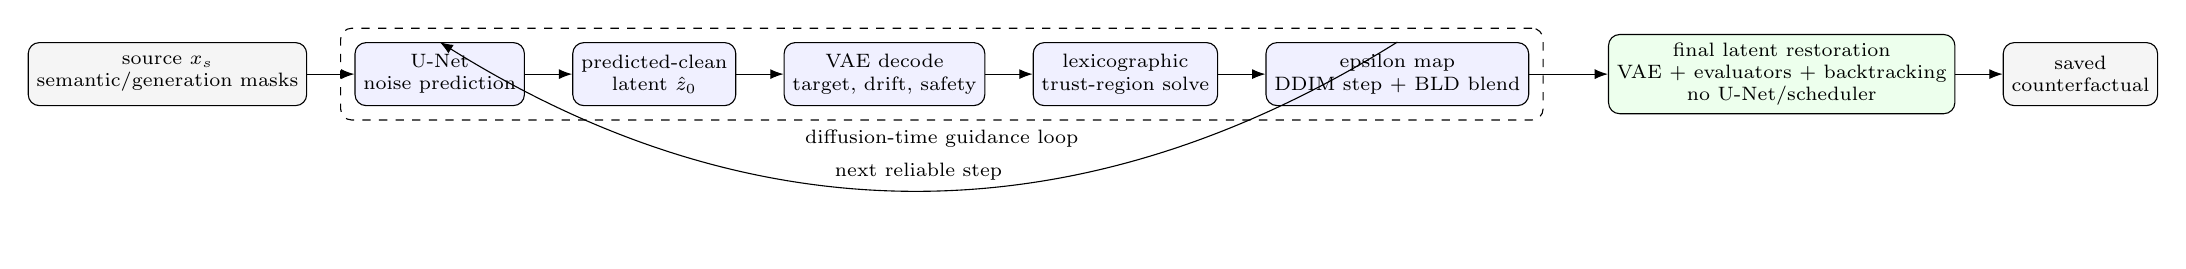
\begin{tikzpicture}[
  node distance=5mm and 6mm,
  >=Latex,
  box/.style={draw,rounded corners,align=center,font=\scriptsize,
              minimum height=8mm,inner sep=3pt},
  data/.style={box,fill=gray!8},
  op/.style={box,fill=blue!6},
  final/.style={box,fill=green!7},
  group/.style={draw,dashed,rounded corners,inner sep=5pt}
]
\node[data] (source) {source $x_s$\\semantic/generation masks};
\node[op,right=of source] (unet) {U-Net\\noise prediction};
\node[op,right=of unet] (clean) {predicted-clean\\latent $\hat z_0$};
\node[op,right=of clean] (measure) {VAE decode\\target, drift, safety};
\node[op,right=of measure] (solve) {lexicographic\\trust-region solve};
\node[op,right=of solve] (sched) {epsilon map\\DDIM step + BLD blend};
\node[final,right=10mm of sched] (restore) {final latent restoration\\VAE + evaluators + backtracking\\no U-Net/scheduler};
\node[data,right=of restore] (output) {saved\\counterfactual};

\draw[->] (source) -- (unet);
\draw[->] (unet) -- (clean);
\draw[->] (clean) -- (measure);
\draw[->] (measure) -- (solve);
\draw[->] (solve) -- (sched);
\draw[->] (sched) -- (restore);
\draw[->] (restore) -- (output);
\draw[->,bend left=32] (sched.north) to node[above,font=\scriptsize]
  {next reliable step} (unet.north);
\node[group,fit=(unet)(clean)(measure)(solve)(sched),
      label={[font=\scriptsize]below:diffusion-time guidance loop}] {};
\end{tikzpicture}
}
\caption{\textbf{Method overview.} A11 evaluates target and preservation on a
predicted-clean decode, solves a clean-latent lexicographic trust-region
problem, maps the accepted displacement to epsilon prediction, and continues
DDIM plus source blending. Final restoration is a distinct post-denoising
latent optimization; it reuses the fixed VAE and evaluators but performs no
new U-Net or scheduler transition.}
\label{fig:method}
\end{figure*}

\subsection{Preservation-Aware Final Restoration}

The final \bld{} latent may remain below the target threshold because a local
step is attenuated by the scheduler or source blend. A11 therefore runs at most
12 restoration iterations on the actual post-blend latent. Each iteration
recomputes Eqs.~\eqref{eq:envelope}--\eqref{eq:drift-subproblem} through the
fixed decoder and tests fractions $\{1,1/2,1/4,1/8\}$ of the proposed step.

When the target is infeasible, an accepted candidate must strictly improve its
desired probability and must not worsen the best identity/locality envelope
beyond numerical tolerance. Once target and safety are feasible, a candidate
must maintain them and strictly decrease non-target drift. All accepted steps
must remain within a cumulative clean-latent radius. Failure of every fraction
ends restoration. The saved uint8 image is evaluated again because VAE decoding
and quantization can move a boundary-adjacent output.

\section{Experimental Protocol}

\subsection{Completed Clean Study}

We evaluate smile removal (\texttt{Smiling} $1\!\rightarrow\!0$) on
CelebAMask-HQ~\cite{liu2015celeba,lee2020maskgan}. The semantic support is a
fixed perioral union of mouth, upper-lip, and lower-lip components; a dilated
soft generation mask is used for gradients and \bld{} blending. Two random
cohorts contain 100 completed sources each. Their 200 source IDs are disjoint
across cohorts and paired across methods. Each source produces one output; no
candidate reranking or post-generation attack is used.

All arms use the local Stable Diffusion 2.1 base checkpoint, DDIM, $512^2$
resolution, 35 scheduler steps, classifier-free guidance 5.0, blend start
fraction 0.25, seed 42, float32 MPS execution, and batch size one. The desired
in-loop target probability is 0.8. A11 uses initial/minimum/maximum clean
radii $0.15/0.01/0.30$, target progress fraction $0.9$, reliability alpha
threshold $0.10$, Huber transition $0.02$, at most 12 final iterations, and
cumulative final radius $1.8$.

We compare:
\begin{itemize}
 \item \textbf{A0 BLD}: source blending with no CCI update;
 \item \textbf{A10 fixed}: a fixed nominal gradient composition with the same
       clean-coordinate, constraint, and final-restoration budgets;
 \item \textbf{A11 adaptive}: the proposed lexicographic optimizer.
\end{itemize}

\paragraph{Metrics.}
Target@0.8 is the fraction reaching the declared desired probability 0.8 under
the explained classifier; it is stricter than flip rate at the 0.5 decision
boundary. Identity is the source/output FaceNet cosine. Outside MAE is the
strict outside-mask RGB error on the $[0,255]$ scale. NT drift is the mean
absolute source/output probability change over all 39 non-target attributes;
unlike Eq.~\eqref{eq:drift}, it is reported without Huber smoothing. Runtime is
the median per-image wall time. FR and NT drift use the same frozen multi-label
classifier that guides A10/A11. This is deliberate explained-model evaluation,
not independent-oracle validation.

\subsection{Planned End-to-End Attacked Study}

The pending end-to-end protocol compares A0 and A11 on 300 paired images with
mouth-only support, then on the same 300 IDs with mouth, upper-lip, and
lower-lip support. It includes the localized smooth boundary attack and will
report FID, spatial FID (sFID), face verification accuracy (FVA), feature
similarity (FS), mean number of altered concepts (MNAC), collateral distance
(CD), counterfactual output score (COUT), and FR. The same frozen multi-label
classifier supplies COUT, FR, MNAC, and CD, as well as attack and CCI guidance.
Partial-cohort values are not inserted into this manuscript.

\section{Results}

\subsection{Clean A0/A10/A11 Comparison}

\begin{table*}[t]
\centering
\caption{Completed clean smile-removal comparison over 200 unique paired
sources. Target@0.8 is in percent; Outside is strict outside-mask MAE on $[0,255]$;
Time is median seconds per image. Lower NT drift, Outside, and Time are better;
higher Target@0.8 and Identity are better.}
\label{tab:clean}
\begin{tabular}{lrrrrr}
\toprule
Method & Target@0.8 $\uparrow$ & Identity $\uparrow$ & Outside $\downarrow$ &
NT drift $\downarrow$ & Time $\downarrow$ \\
\midrule
A0 BLD
 & \RawBLDTargetPassRatePct
 & \RawBLDIdentityCosine
 & \RawBLDOutsideMAE
 & \RawBLDNonTargetDrift
 & \RawBLDRuntimeMedian \\
A10 fixed CCI
 & \FixedCCITargetPassRatePct
 & \FixedCCIIdentityCosine
 & \FixedCCIOutsideMAE
 & \FixedCCINonTargetDrift
 & \FixedCCIRuntimeMedian \\
A11 adaptive CCI
 & \AdaptiveCCITargetPassRatePct
 & \AdaptiveCCIIdentityCosine
 & \AdaptiveCCIOutsideMAE
 & \AdaptiveCCINonTargetDrift
 & \AdaptiveCCIRuntimeMedian \\
\bottomrule
\end{tabular}
\end{table*}

Table~\ref{tab:clean} shows the intended fixed/adaptive comparison. A11 lowers
NT drift by \AdaptiveDriftReductionVsFixedPct\% relative to A10
(\AdaptiveCCINonTargetDrift{} versus \FixedCCINonTargetDrift) while its
Target@0.8 rate is one percentage point lower
(\AdaptiveCCITargetPassRatePct\% versus \FixedCCITargetPassRatePct\%). Mean
identity differs by $0.0034$ and outside MAE by
$0.0057$ on the $[0,255]$ scale. Thus the saved cohort supports reduced
collateral movement at a closely matched, but not identical, target operating
point. It does not establish statistical superiority because this table does
not include a paired confidence interval.

Both guided methods substantially increase Target@0.8 over A0 and also increase mean
identity cosine in this cohort. This does not mean A0 was optimized for lower
identity; A0 simply performs the substantially cheaper \bld{} path. A11's
median runtime is \AdaptiveCCIRuntimeMedian{} s versus
\FixedCCIRuntimeMedian{} s for A10 and \RawBLDRuntimeMedian{} s for A0. The
extra cost comes from repeated VAE decodes, evaluator forwards/backwards, and
candidate evaluations during final restoration; the small active-set solve is
not the dominant cost.

\subsection{Illustrative Final-Restoration Ablation}

\begin{table}[t]
\centering
\caption{Mechanism ablation for source \RestorationSampleID. This single case
illustrates what restoration can do; it is not population evidence.}
\label{tab:restoration}
\begin{tabular}{lrr}
\toprule
Metric & Without & With \\
\midrule
Desired probability & \RestorationBeforeProbability & \RestorationAfterProbability \\
Identity cosine & \RestorationBeforeIdentity & \RestorationAfterIdentity \\
NT drift & \RestorationBeforeDrift & \RestorationAfterDrift \\
Runtime (s) & \RestorationBeforeRuntime & \RestorationAfterRuntime \\
\bottomrule
\end{tabular}
\end{table}

For source \RestorationSampleID, restoration accepts
\RestorationAcceptedSteps{} steps and raises desired probability from
\RestorationBeforeProbability{} to \RestorationAfterProbability{} while
identity increases from \RestorationBeforeIdentity{} to
\RestorationAfterIdentity{} (Table~\ref{tab:restoration}). NT drift also rises
from \RestorationBeforeDrift{} to \RestorationAfterDrift, exposing the cost of
recovering a severely missed target. The final image differs from the
no-restoration output by pixel MAE \RestorationPixelMAE, maximum normalized
change \RestorationPixelMax, and \RestorationChangedPct\% changed pixels. This
example validates the acceptance mechanism and its locality, not an average
benefit.

\subsection{Pending End-to-End Results}

\begin{table*}[t]
\centering
\caption{End-to-end attacked evaluation with mouth-only support. The cohort
will contain 300 paired images; partial values are intentionally omitted.}
\label{tab:attacked-mouth}
\begin{tabular}{lrrrrrrrr}
\toprule
Method & FID $\downarrow$ & sFID $\downarrow$ & FVA $\uparrow$ & FS $\uparrow$ &
MNAC $\downarrow$ & CD $\downarrow$ & COUT $\uparrow$ & FR (\%) $\uparrow$ \\
\midrule
A0 BLD & \multicolumn{8}{c}{Pending (300-image run)} \\
A11 adaptive CCI & \multicolumn{8}{c}{Pending (300-image run)} \\
\bottomrule
\end{tabular}
\end{table*}

\begin{table*}[t]
\centering
\caption{End-to-end attacked evaluation with mouth, upper-lip, and lower-lip
support on the same 300 IDs. Partial values are intentionally omitted.}
\label{tab:attacked-lips}
\begin{tabular}{lrrrrrrrr}
\toprule
Method & FID $\downarrow$ & sFID $\downarrow$ & FVA $\uparrow$ & FS $\uparrow$ &
MNAC $\downarrow$ & CD $\downarrow$ & COUT $\uparrow$ & FR (\%) $\uparrow$ \\
\midrule
A0 BLD & \multicolumn{8}{c}{Pending (300-image run)} \\
A11 adaptive CCI & \multicolumn{8}{c}{Pending (300-image run)} \\
\bottomrule
\end{tabular}
\end{table*}

\section{Limitations}

The completed study covers one facial attribute, one dataset, one diffusion
backbone, a fixed perioral policy, and deterministic seed-42 generation. Its
200-image statistics are descriptive and do not include identity-cluster
bootstrap intervals. The fixed and adaptive operating points are close but not
exactly equal in FR; a calibrated matched-success frontier would support a
stronger comparison.

The same classifier guides generation and supplies FR and NT drift. This is
appropriate when the object of explanation is that classifier, but it can
reward classifier-specific features and cannot establish semantic agreement
for another model or for people. The pending COUT, FR, MNAC, and CD metrics
share this limitation by design. Independent transfer and human evaluation are
future validation, not claims of this draft.

The local linearized problems provide an auditable priority rule, not a global
convergence guarantee for a changing non-convex diffusion trajectory. Mask
quality also bounds the meaning of locality: segmentation errors may omit
relevant evidence or admit unrelated pixels. Runtime is several times that of
A0 because VAE/evaluator differentiation and restoration line searches are
serial on MPS.

Finally, facial images and identity embeddings are biometric data. This method
should be used for consented model auditing with appropriate data protection,
not for inferring sensitive traits or modifying identity documents. A model
counterfactual must be disclosed as generated evidence about a classifier, not
as a plausible real-world causal statement.

\section{Conclusion}

\method{} replaces a permanent weighted objective with an explicit local
ordering: make attainable target progress, minimize unavoidable identity and
locality violation, then reduce non-target drift. Predicted-clean measurements
place heterogeneous evaluators on an image estimate, clean-coordinate trust
regions remove scheduler-dependent step units, and final restoration applies
the same priorities to the actual post-\bld{} latent. On 200 completed paired
smile-removal sources, A11 reduces non-target drift by
\AdaptiveDriftReductionVsFixedPct\% relative to matched fixed A10 at a
one-point lower Target@0.8 rate, with nearly unchanged identity and outside-mask error but
higher runtime. The pending 300-image attacked studies will determine whether
that advantage persists in the full end-to-end protocol.

\bibliographystyle{plain}
\bibliography{references}

\end{document}
